\documentclass[PMO,authoryear,toc]{lsstdoc}
\usepackage{ragged2e}
% lsstdoc documentation: https://lsst-texmf.lsst.io/lsstdoc.html
%\input{meta}

% Package imports go here.

% Local commands go here.

%If you want glossaries
%\input{aglossary.tex}
%\makeglossaries

\title{Virtualization Cluster Topology and Design}

% Optional subtitle
% \setDocSubtitle{A subtitle}

\author{%
Heinrich Reinking
}

\setDocRef{ITTN-036}
\setDocUpstreamLocation{\url{https://github.com/lsst-it/ittn-036}}

\date {\today}

% Optional: name of the document's curator
% \setDocCurator{The Curator of this Document}

\setDocAbstract{%
The following document lays out the design and topology of the virtualization cluster of Rubin Observatory locations, base, summit, and Tucson.
}

% Change history defined here.
% Order: oldest first.
% Fields: VERSION, DATE, DESCRIPTION, OWNER NAME.
% See LPM-51 for version number policy.
\setDocChangeRecord{%
  \addtohist{1}{2021-02-10}{First Commit}{Heinrich Reinking}
  \addtohist{2}{2021-03-05}{First Revision Concluded}{Heinrich Reinking}
  \addtohist{3}{2021-10-12}{LaTeX conversion and Document Update}{Heinrich Reinking}
}


\begin{document}

% Create the title page.
\maketitle
% Frequently for a technote we do not want a title page  uncomment this to remove the title page and changelog.
% use \mkshorttitle to remove the extra pages

% ADD CONTENT HERE
% You can also use the \input command to include several content files.
\section{Introduction}
\justify{The following document lays out the design and topology of the virtualization cluster of Rubin Observatory locations, base, summit, and Tucson.}

\section{Motivation}
\justify{New technologies and developments are developed at an unprecedented pace. Virtualization became a standard for the industry many years ago, but it has been replaced by new technologies, like micro-services and containerize applications; however, there are still some services that need to be run in VM.}
\justify{The following are some of the critical services for Rubin Observatory that are required to run in virtual machines:}

\begin{itemize}
  \item Several Windows servers such as Domain Controllers, Email, etc.
  \item HVAC Controlling Platform system at the Summit
  \item Fire Detection system at the Summit
  \item The UPS platform at the summit
  \item Cisco services such as the Wireless Lan Controller, Cisco Unified Communications Manager, etc.
\end{itemize}
\justify{Virtualization also provides an extra layer of availability for services running on containers.}

\newpage
\section{Requirements}
\justify{Clusters must meet the following criteria and recommendations:}

\begin{itemize}
  \item Front-end Graphical User Interface for easy VMs creation, manipulation, edition, and deletion.
  \item Connection to a centralized authentication backend, such as LDAP, OpenLDAP or FreeIPA.
  \item The cluster size has to be an odd number.
  \item Reliable support or at least wide community support.
  \item A common storage pool that all cluster nodes can access at all time.
  \item The storage pool has to be able to tolerate catastrophic events, such as disk failures, servers maintenance, failures, and network outages.
  \item Each hypervisor must enter maintenance, allowing all services and Virtual Machines to remain ongoing on a different hypervisor of the cluster.
  \item If a node is abruptly taken offline, the Virtual Machines running in such node must be able and capable of live auto-migration.
  \item If a node irrevocably shuts down - complete hardware failure - the node must be easily replaced with a new one, with no data corruption.
\end{itemize}

\newpage
\section{OpenSource vs Licenced Solution}
\justify{There are several alternatives to deploy a Virtualization Server and another few for Virtualization Clusters. For this document, we'll be grouping them into two big groups OpenSource - no license or support cost, with support from the OpenSource community - and the Licenced ones - license and support cost.}

\newpage
\subsection{OpenSource}
\justify{For the OpenSource analysis, we'll be using QEMU. QEMU - short for Quick EMUlator - is a generic open-source machine emulator and virtualizer. When used as a virtualizer, it is commonly used with KVM - Kernel-based Machine - which can virtualize x86, server and embedded PowerPC, 64-bit POWER, S390, 32-bit, and 64-bit ARM, and MIPS guests.}

In terms of requirements:

\begin{itemize}
  \item QEMU does have a GUI called Virtual Manager that allows you to manage VMs running across the cluster.
  \item The problem is the access: get to it, you need to either export display through an ssh session or access through remote desktop to the primary Hypervisor. Also, simultaneous user access isn't doable, but it can be accomplished through third-party applications, like VNC.
  \item QEMU does not allow remote authentification directly into the Virtual Manager, but it can be done through third-party applications.
  \item QEMU allows live migration - with a shared storage pool - but does not have any live-auto migration feature. This means that if a node shuts down or fails, the VM will fail as well, and it will not be loaded in another server. Also, if the node is lost for good, the VM will have to be recreated in KVM, but the OS and the data will remain cause the VM's Virtual Drive is in the shared storage pool.
  \item Since live migration is an option, then a node can be taken offline for maintenance or replacement, without outages or downtime required.
  \item The fact that is OpenSource has its advantages and disadvantages. On the Pro side, you have an entire community constantly checking for bugs and also supporting you in case your instance fails, as well as a lot of information online. The Con, OpenSource software is vulnerable to glitches and bugs, and even though there is a whole community to support since you are not paying for service, no one is obligated to respond or help.
  \item If used without a common storage pool and only local server storage, it raises a big risk, cause not only live migration is not an option but if the server and/or local storage fails, the Virtual Machine is lost for good, representing a dangerous Single Point of Failure (SPF).
\end{itemize}

\newpage
\subsection{VMWare}
\justify{For the licenced solution, we are going to analyze VMWare's solution: vSphere + vCenter + vSAN. vSphere is a compute virtualization platform, which along with vCenter, it allows to control multiple Virtualization Servers - that are running vSphere. VMWare offers all amount of services and features, which goes hand by hand with the costs.}

In terms of requirements:
\begin{itemize}
  \item It offers a front-end Web User Interface (WUI) through the vCenter Server. This allows management, migration, creation, modify or delete VMs, as long as several other services.
  \item Offers a connection to remote Centralized Authentication Platforms.
  \item It has a feature called vMotion, which allows live-auto migration, meaning that if a node is scheduled for maintenance or powered off, the VM will automatically be redeployed in another node.
  \item It comes with three-year support, which includes 24/7 online helpdesk and software updates.
  \item vCenter requires a Common Storage Pool to enable the live-auto migration feature.
  \item Virtual SAN or vSAN is a logical partition in a physical storage area network (SAN) \footnote{https://searchstorage.techtarget.com/definition/virtual-storage-area-network}. This allows vCenter to have a common Storage Pool to permit live migration.
\end{itemize}

\newpage
\section{Design}
\justify{VMWare is a paid service, so support and guarantee give us a relatively bug-free environment, eventhough QEMU is capable of almost everything that vSphere can, it's not recommended for an industrial usability; specially since the purpose of this cluster is to support and run essential/core services, we must be able to guarantee that neither the servers or storage represents a SPF. Taking under consideration both the benefits and disadvantages of both schemes, the proposed desgined is over VMWare.}

\begin{figure}
  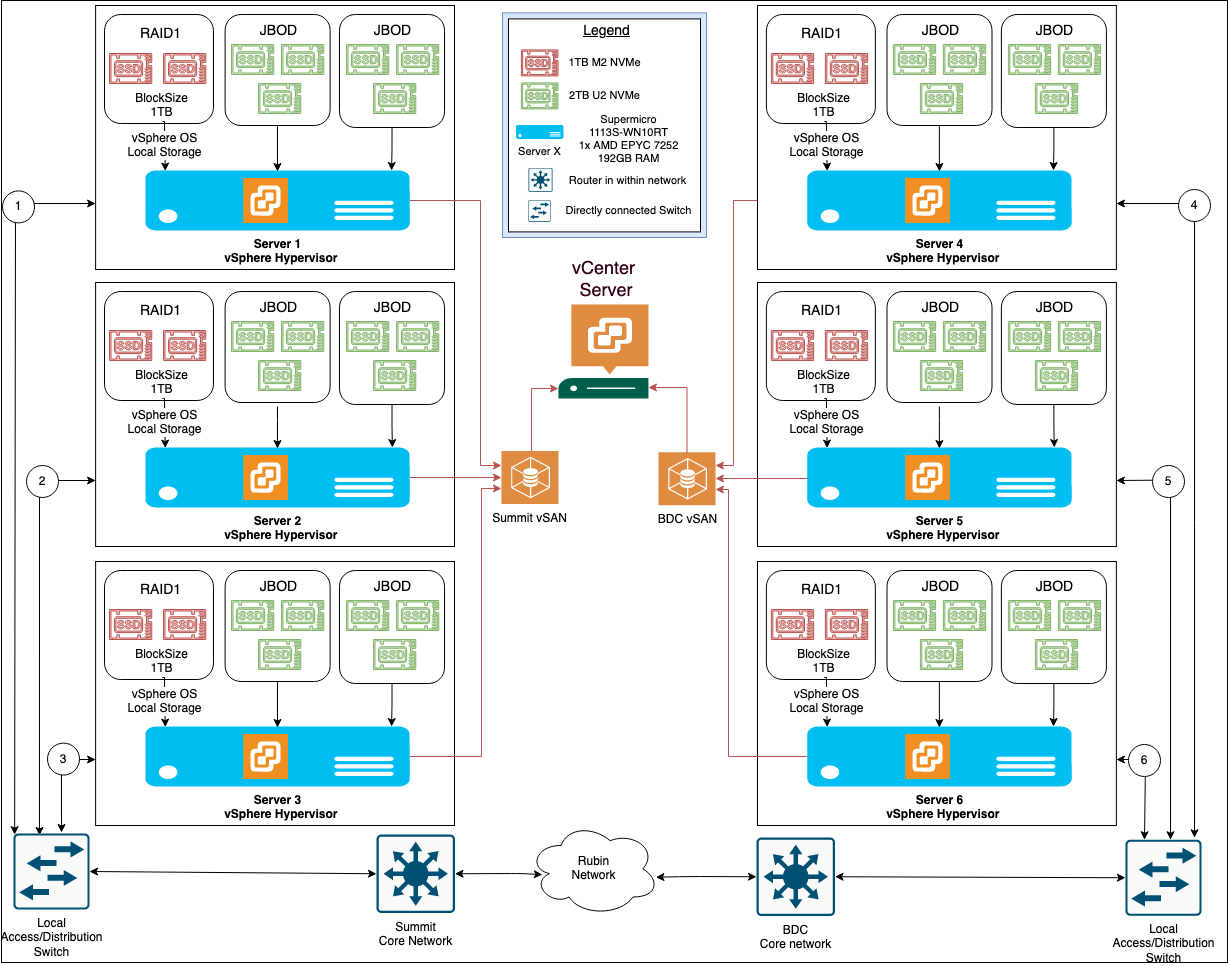
\includegraphics[width=12cm]{images/vmware_cluster_design.png}
  \centering
  \caption{VMWare Cluster Design}
\end{figure}

\begin{itemize}
  \item The OS (ESXi or vSphere) is mounted over a RAID1, construct over 2x1TB NVMe M.2.
  \item 3 x 2TB U.2. NVMe Drives, JBOD configured, passing through all drives to vSAN.
  \item Dedicated network for vSAN and other for vMotion, per site.
  \item One cluster per site, each with 3 Servers, with separate vSAN pools.
  \item One vCenter Server handling both clusters.
  \item A DSwitch (Distributed Switch) for vMotion and another for vSAN, per site.
\end{itemize}

\newpage
\section{Failover and WCS}
\justify{WCS stands for Worst Case Scenario. The suggested design takes under consideration the following scenarios:}

\subsection{System Disk Failure}
\justify{In the first scenario, we considered the loss of one of the two System Disks. By System Disks, we are referring to the drives from where the OS is mounted.}
\begin{figure}
  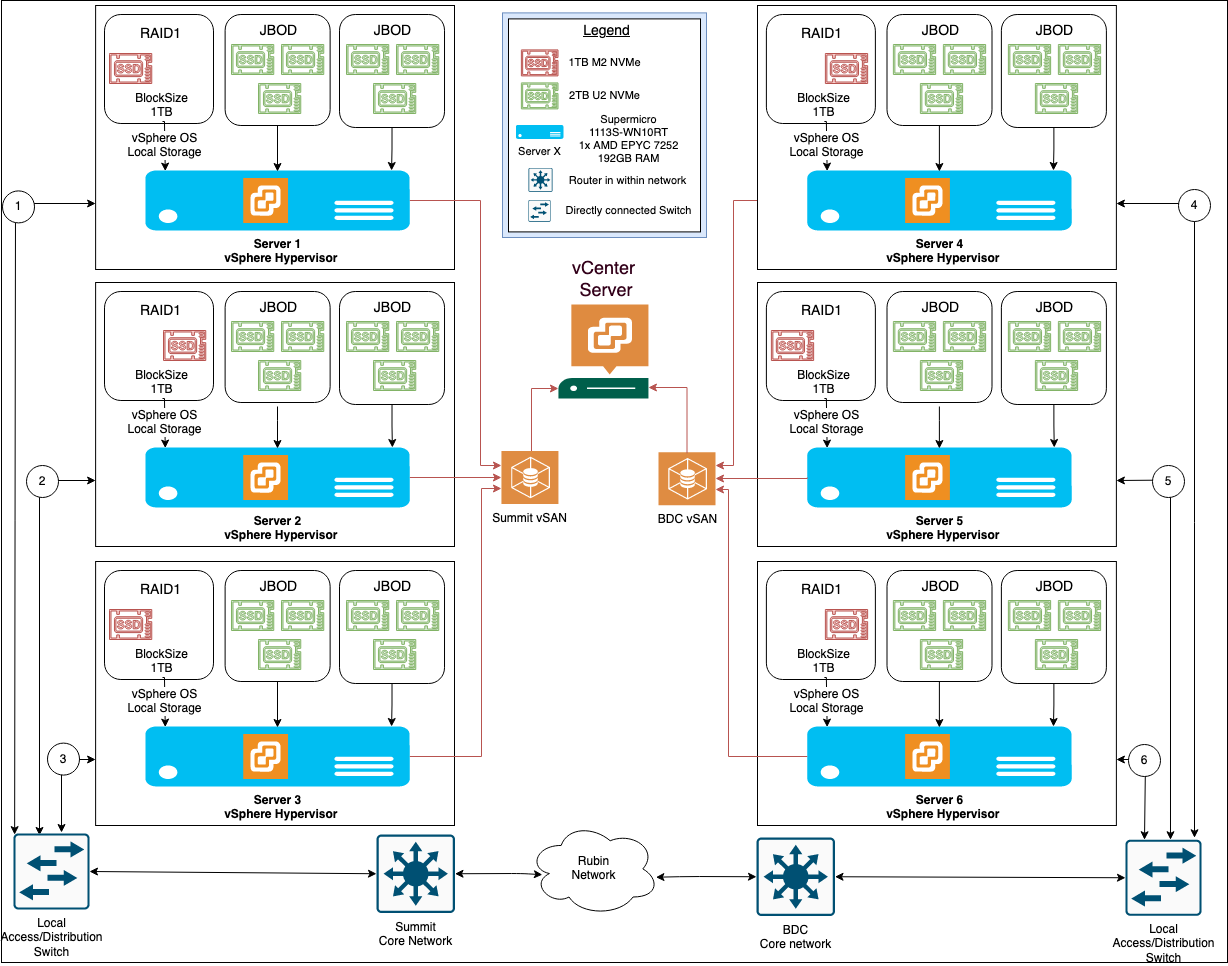
\includegraphics[width=10cm]{images/system_disk_failure.png}
  \centering
  \caption{System Disk Failure}
\end{figure}
\justify{Since the System Disks are set up in RAID1, the system will continue to go one, and hot-swap can be performed to replace the failed drive. No downtime is needed.}

\newpage
\subsection{Data Disks or Server Failure}
\justify{The Data disk consists of where the Virtual Machines Virtual Drives allocate. Virtual Drive is a logical drive created by the virtualization agent, which reserves a space disk on the shared storage, but from the VM perspective, it is a regular drive.}

\begin{figure}
  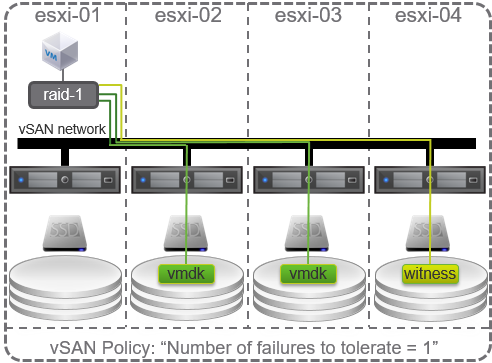
\includegraphics[width=8cm]{images/data_disk_failure.png}
  \centering
  \caption{Data Disk Failure}
\end{figure}

\newpage
\justify{vSAN is configured with toleration one or RAID1 \footnote{https://www.definetomorrow.co.uk/blog/2017/9/22/vmware-vsan-a-closer-look-data-availabilty}. As seen in the attached schematic, each disk has a replica on other servers, meaning that either one server or 1 data disk (per server) can be lost, and everything would remain operational with no downtime.}
If 2 servers are to be down or lost, vSAN goes into Read-Only mode.

\begin{figure}
  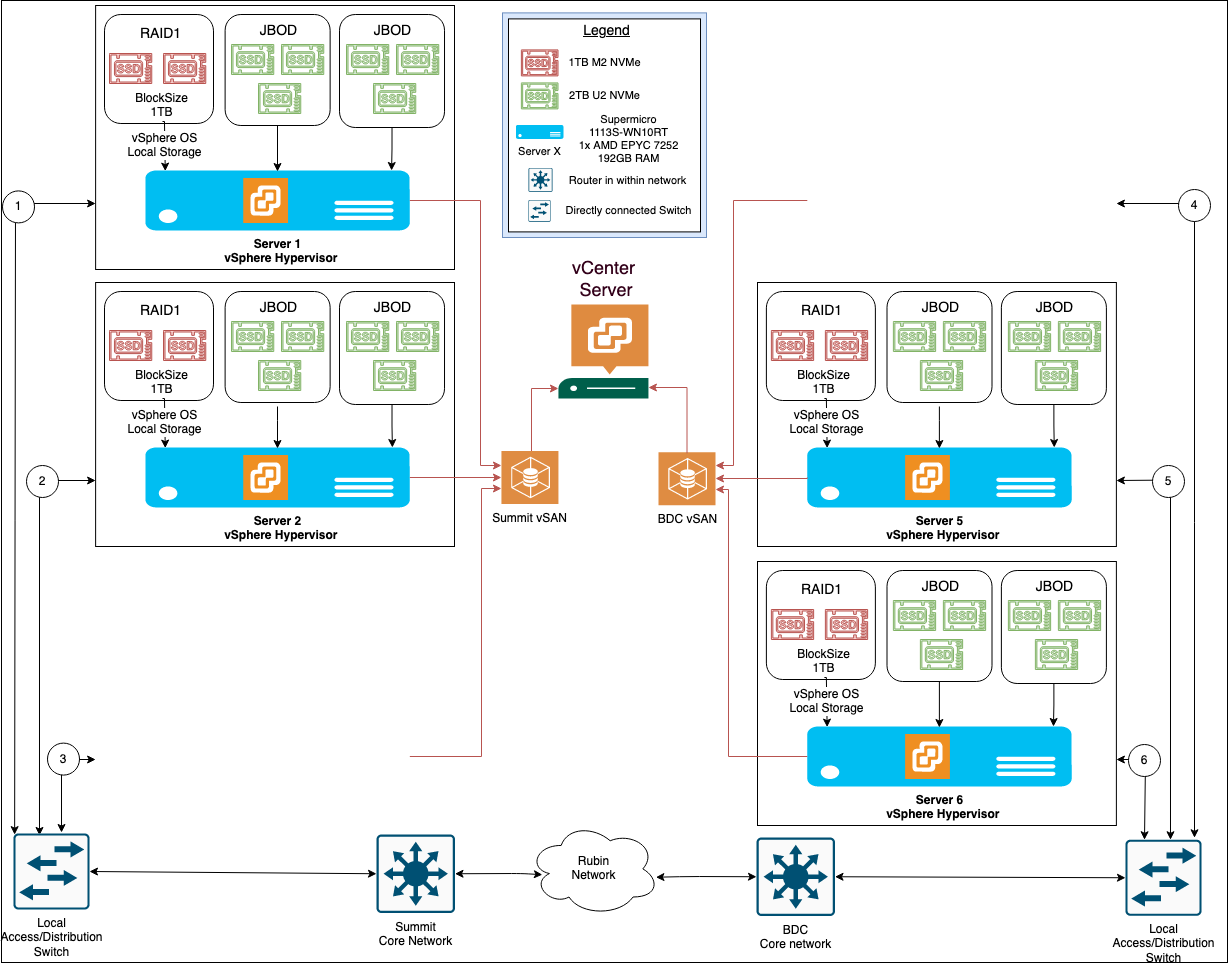
\includegraphics[width=12cm]{images/server_failure.png}
  \centering
  \caption{Server Loss or Failure}
\end{figure}

\subsection{Network Outage}
\justify{Over the Summit, each link - 1, 2, and 3- are composed of 2 connections: A primary and failover; the same goes for the BDC connections 4 5, and 6. These are not PC (Port-Channel) nor VPC (Virtual Port-Channel), but a failover handled by each vSphere, meaning that if the primary link is lost, the failover kicks in.}
\justify{If both links are lost, we face a similar scenario to a Server Loss with one difference: The VM's in the lost node will migrate to another running hypervisor. When the node is back online, vCenter and vSAN will detect a leftover VM running in the node, destroy it, and update the Objects Database.}



\appendix
% Include all the relevant bib files.
% https://lsst-texmf.lsst.io/lsstdoc.html#bibliographies
\renewcommand{\refname}{} % Suppress default Bibliography section
\bibliography{local,lsst,lsst-dm,refs_ads,refs,books}

% Make sure lsst-texmf/bin/generateAcronyms.py is in your path
\section{Acronyms} \label{sec:acronyms}
\newpage
\addtocounter{table}{-1}
\begin{longtable}{p{0.145\textwidth}p{0.8\textwidth}}\hline
\textbf{Acronym} & \textbf{Description}  \\\hline

BDC & Base Data Center \\\hline
KVM & Kernel-based Virtual Machine \\\hline
LDAP & Lightweight Directory Access Protocol \\\hline
VM & Virtual Machine \\\hline
VNC & Virtual Network Computing \\\hline
vSAN & Virtual Storage Area Network \\\hline
\end{longtable}

% If you want glossary uncomment below -- comment out the two lines above
%\printglossaries





\end{document}
